\begin{enumerate}[label=\thesection.\arabic*.,ref=\thesection.\theenumi]
\numberwithin{equation}{enumi}
\item
Consider a unity feedback system as shown in the figure,shown with an integral compensator k/s and open-loop transfer function
\begin{align}
G(s) = \frac{1}{s^2+3s+2}
\end{align}
where k greater than 0. The positive value of k for which there are two poles of unity feedback system on j${\omega}$ axis is equal to-----(rounded off to two decimal places)
\centering
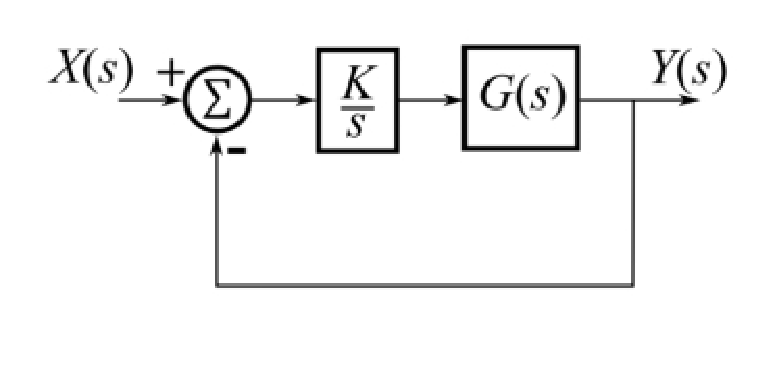
\includegraphics[width=\columnwidth]{./figs/ee18btech11005.eps}
\\
\solution The transfer function for negative feedback is given by
\begin{align}
\frac{Y(s)}{X(s)} &= \frac{G(s)}{1+G(s)H(s)}
\end{align}
where H(s) = 1 for unity feedback system
and G(s) is net forward open loop gain
\\
\begin{align}
G(s) &=  \sbrak{\frac{1}{s^2+3s+2}}\sbrak{\frac{k}{s}}
&= \frac{k}{s^3+3s^2+2s}
\end{align}
Characteristic equation is..,
\\
\begin{align}
 1 + G(s)H(s) = 0 \label{eq:sec_order_op}
\\
=> 1 + \sbrak{\frac{k}{s^3+3s^2+2s}} = 0
\\
=> s^3+3s^2+2s+k = 0
\end{align}
The Routh hurwitz criterion:-
\\
This criterion is based on arranging the coefficients of characteristic equation into an array called Routh array.
\\
For any characteristic equation q(s),
\\
\begin{align}
q(s) = a_0s^n+a_1s^{n-1}+a_2s^{n-2}+.....+a_{n-1}s+a_n = 0
\end{align}
Routh array can be constructed as follows..,
\begin{vmatrix} s^n\\s^{n-1}\\s^{n-2} \\ \vdots \end{vmatrix} \begin{vmatrix}
a_0 & a_2 & a_4 & \cdots \\
a_1 & a_3 & a_5 & \cdots  \\
b_1 & b_2 & b_3 & \cdots \\
\vdots & \vdots & \vdots & \ddots &\vdots 
 \cdots \\ \end{vmatrix}
 \\
 where
 \begin{align}
 b_1 =\frac{ a_1a_2-a_0a_3}{a_1}  
 \\
 b_2 =\frac{ a_1a_4-a_0a_5}{a_1} 
 \\
 c_1=\frac{ b_1a_3-a_1b_2}{b_1} 
\\
 c_2=\frac{ b_1a_5-a_1b_3}{b_1}  
\end{align}
\\
For poles to lie on imaginary axis any one entire row of hurwitz matrix should be zero.
\\ Constructing the routh array for the characteristic equation obtained in equation(\ref{eq:sec_order_op})
\begin{align}
 s^3+3s^2+2s+k = 0
\end{align}
%
%\begin{lstlisting}
%codes/ee18btech11002/plot.py
%\end{lstlisting}
\begin{align}
\begin{vmatrix}s^3\\s^2\\s^1 \\ s^0 \end{vmatrix} \begin{vmatrix}
1 & 2 \\ 3 & k \\  \frac{6-k}{3} & 0\\ k & 0
\end{vmatrix}
\end{align}
\\
For poles on j$\omega$ axis any one of the row should be zero.
\\
\begin{align}
\frac{6-k}{3} = 0 \hspace{5pt} or\hspace{5pt} k = 0
\end{align}
\\
But given k greater than 0 ...
\begin{align}
   6-k = 0\\
   k = 6
\end{align}
\end{enumerate}
Y(s) = Z(s).G(s)
\newline 
Z(s) = X(s) - Y(s).H(s) => X(s) = Z(s)+Y(s).H(s)
\newline
X(s) = Z(s)+Z(s).G(s).H(s)
\newline 
$\frac{Y(s)}{X(s)}$ = $\frac{Z(s).G(s)}{Z(s)+Z(s).G(s).H(s)}$

So,the transfer function of negative feedback is $\frac{G(s)}{1+G(s).H(s)}$
\newline Since unit feedback H(s) = 1
\newline Now the transfer function of unity negative feedback is $\frac{G(s)}{1+G(s)}$
\end{frame}
\begin{frame}{Net transfer function}
  The net transfer function in the given question is.....
  \newline
  
  $\frac{Y(s)}{X(s)}$ = $\frac{G(s)*k/s}{1+G(s)*k/s}$
  \newline
  
  The characteristic equation is 1 + (G(s)x$\frac{k}{s}$) = 0
 \newline that is..,
 \newline 
 
 C.E = 1 + $\frac{k}{s(s^2+3s+2)}$ = 0
 =>s(s^2+3s+2) + k = 0
 \newline 
 
=> s^3+3s^2+2s+k=0
 \end{frame}
 \begin{frame}{Routh-Hurwitz Criterion}
 This criterion is based on arranging the coefficients of characteristic equation intoan array called Routh array.
 \newline
 
 q(s) = $a_0$s^n+$a_1$s^{n-1}+$a_2$s^{n-2}+.....+$a_{n-1}$s+$a_n$ = 0
\newline 

\begin{vmatrix}s^n\\s^{n-1}\\s^{n-2} \\ \vdots \end{vmatrix} \begin{vmatrix}
a_0 & a_2 & a_4 & \cdots \\
a_1 & a_3 & a_5 & \cdots  \\
b_1 & b_2 & b_3 & \cdots \\
\vdots & \vdots & \vdots & \ddots &\vdots 
 \cdots \\ \end{vmatrix} where b_1 =\frac{ a_1a_2-a_0a_3}{a_1}  \hspace{5pt} b_2 =\frac{ a_1a_4-a_0a_5}{a_1} \hspace{5pt} c_1=\frac{ b_1a_3-a_1b_2}{b_1}  \hspace{5pt}     c_2=\frac{ b_1a_5-a_1b_3}{b_1}  
 \end{frame}
 \begin{frame}
 For poles to lie on imaginary axis any one entire row of hurwitz matrix should be zero.
 \newline 
 
 For the given characteristic equation =  s^3+3s^2+2s+k = 0
 \newline \begin{vmatrix}s^3\\s^2\\s^1 \\ s^0 \end{vmatrix} \begin{vmatrix}
1 & 2 \\ 3 & k \\  \frac{6-k}{3} & 0\\ k & 0
\end{vmatrix}
\newline $For poles on $j$\omega$ axis any one of the row should be zero
\newline => $\frac{6-k}{3}$ = 0 or k = 0
\newline But given k>0 ...
\newline therefore, 6-k=0 => k = 6
\end{frame} 
\begin{frame}
To find the location of poles on j$\omega$ axis 
\newline 

Auxillary equation of the given CE is 3s^2 + k = 0
\newline
=> 3s^2 + 6 = 0
\newline
=> s = \pm j2
    
\end{frame}     
\end{document}
